\chapter{Analyse des performances du \texorpdfstring{$3\times 1\times 1$}{3x1x1}}\label{chap::5}
    \chapterprecishere{
        ``Potentielle citation sans aucun rapport avec le sujet"\par\raggedleft--- \textup{Personne inconnue}, contexte à déterminer
    }
    
  \section{Introduction}
    % obj
    Le prototype de \gls{dlartpc} de \TOO{}, premier prototype du projet \protodp{}, a pris des données au \gls{cern} entre Juin et Novembre 2017. Son objectif premier était de vérifier que la solution \gls{dlartpc} est réalisable à grande échelle et de tester les choix technologiques en vue de la construction du démonstrateur de \SSS{}. De plus, grâce aux données de muons cosmiques récoltées, le \TOO{} peut estimer le gain et regarder sa stabilité au cours du temps et à travers la grande surface de son \gls{crp}. Il peut également regarder l'évolution du gain en fonction du champ dans les \glspl{lem}, mesures qui peuvent alors être comparées à celles effectuées en 2014 dans le prototype de \threeL\cite{Cantini2014}. Ce sont ces derniers points qui sont traités en détail dans ce dernier chapitre.

    Le \TOO{} a rencontré un problème majeur qui l'a empêché de fonctionner au mieux de ses capacités : la grille était limitée en tension à \SI{5}{\kilo\volt}. Ceci a limité les différents champs applicables à travers le \gls{crp}, à savoir les champs d'extraction, d'amplification et d'induction. Cette limitation était due à un groupe de fils mal tendus ainsi qu'à un contact défectueux et ne remet donc pas en cause la technologie \gls{dlartpc}. En effet, malgré ces difficultés, le \TOO{} a démontré la capacité de cette technologies à visualiser avec une grande précision des topologies complexe, comme le montre les quelques traces de la \autoref{fig::data-sample}. Ces événements ont été vus à des champs électriques bien inférieurs aux champs nominaux décrits dans \autoref{sec::TOO-intro}.. Ce problème de limitation en tension à néanmoins fait que le champ d'extraction était faible (de l'ordre de \SI{1}{\kilo\volt\per\centi\meter}) lors de la mesure du gain à des champs d'amplification supérieur à \SI{30}{\kilo\volt\per\centi\meter}. L'analyse des runs correspondant a nécessité le développement d'un algorithme d'analyse dédié.

    Ce chapitre commence par une présentation de la méthode d'analyse en \autoref{sec::methode-analyse} : comment le gain peut être estimé et comment la reconstruction des traces est effectuée par le logiciel LArSoft. Les principales incertitudes systématiques, dominantes par rapport au incertitudes statistiques, sont également présentées. Dans la \autoref{sec::data-311} sont présentées les données utilisées : les dates de mesures et les champs électriques scannés, ainsi que les mesures du slow control (pression, température, niveau de l'interface liquide-gaz). Les résultats de l'analyse de stabilité dans le temps ainsi que des variations de gain sur la surface du \gls{crp} sont présentés en \autoref{sec::results-311}. Y figure aussi l'évolution du gain en fonction du champ électrique dans les \glspl{lem}. Enfin, l'analyse et la reconstruction des données aux champs d'amplification supérieurs à \SI{30}{\kilo\volt\per\centi\meter} et présentée en \autoref{sec::rawdatasoft}.

    \begin{figure}[htpb]
      \centering
      \includegraphics[width=\textwidth]{events.pdf}
      \caption[Quelques événements vus dans le \TOO{}]{\label{fig::data-sample}Quelques agrandissements  d'événements vus dans le \TOO{} à un champ d'extraction de \SI{1.7}{\kilo\volt\per\centi\meter} dans le liquide, un champ d'amplification de \SI{28}{\kilo\volt\per\centi\meter} et un champ d'induction de \SI{1}{\kilo\volt\per\centi\meter}. La colonne de gauche est la vue 0, la colonne de droite est la vue 1. De bas en haut : deux gerbes hadroniques et une gerbe électromagnétique.}
    \end{figure}
  
  \section{Méthode d'analyse}\label{sec::methode-analyse}

    \begin{figure}[htpb]
      \centering
      \includegraphics[width=0.8\textwidth]{crp.png}
      \caption[Schéma du CRP du \TOO{} vue de dessus]{\label{fig::crp-chap5}Schéma du \gls{crp} du \TOO{} vue de dessus.}
    \end{figure}

    \subsection{Mesure du gain effectif}

      Les anodes de lectures du \TOO sont segmentées en deux vues. La vue 0, de $100\times\SI{100}{\centi\meter}$, correspond aux canaux de lecture de \SI{3}{\meter} tandis que la vue 1, de $100\times\SI{300}{\centi\meter}$, correspond aux canaux de lecture de \SI{1}{\meter} (voir \autoref{fig::crp-chap5}). La charge déposée par unité de longueur se répartira de manière équitable entre ces deux vues (les diffusions sont négligeables sur une dérive de \SI{1}{\meter}, voir \autoref{sec::ionisation}), selon une convolution entre une distribution de Landau-Vavilov et une gaussienne (voir \autoref{sec::ionisation}). Un ajustement peut alors être fait pour extraire la valeur de la \gls{mpv} de la distribution de Landau-Vavilov, dont la valeur est connue pour des muons cosmiques, à savoir \SI{8.26}{\femto\coulomb\per\centi\meter} (voir \autoref{tab::muon}). Le gain effectif est alors défini comme le rapport entre la somme des \gls{mpv} de la distribution de la charge dans les deux vues et la \gls{mpv} attendue.

      \subsubsection{Calibration}

        \begin{figure}[htbp]
          \centering
          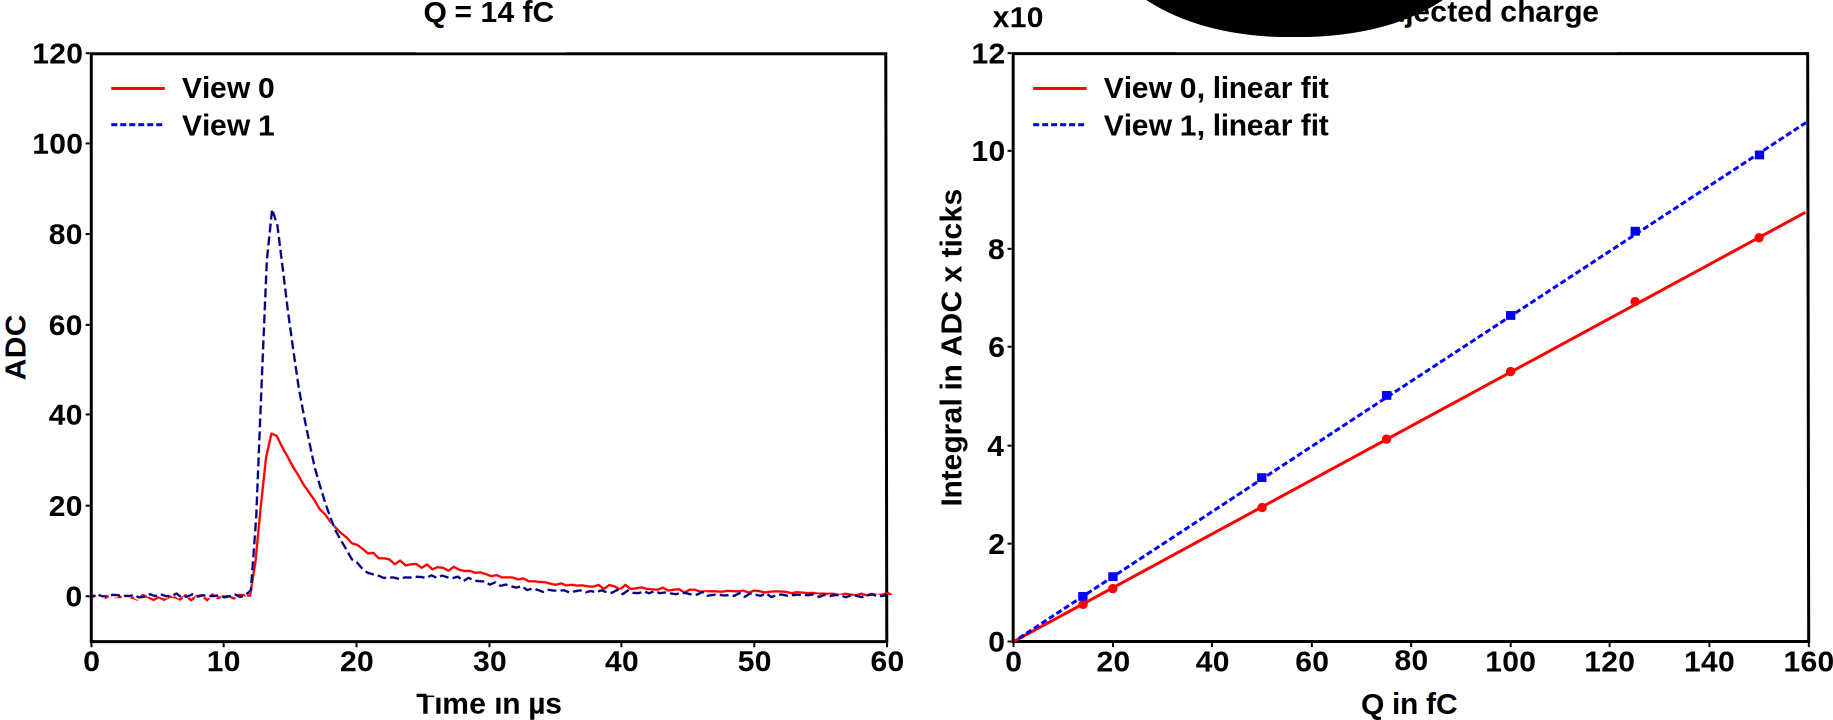
\includegraphics[width=\textwidth,keepaspectratio]{calibration.pdf}
          \caption[Réponse de l'électronique de lecture]{\label{fig::cali-311}Réponse de l'électronique de lecture à des signaux d'intensité variable. À gauche, le signal dans un canal de la vue 0 et un canal de la vue 1, ajustés par l'équation \eqref{eq::resp-function}. À droite, la variation de l'intégrale du signal ajusté en fonction de la charge injectée.}
        \end{figure}

        La réponse de l'électronique de lecture du \TOO{} a été calibrée en envoyant des impulsions d'amplitudes variable à travers les canaux de lecture. Dans le cas où la charge déposée dans un canal de lecture est étiré en temps, l'intégrale du signal correspondant au coup doit être utilisé pour évaluer la charge incidente. Dans une \gls{dlartpc}, le coup peut en effet être étiré en temps à bas champ d'extraction (voir \autoref{sec::extraction}). Le courant $I(t)$ induit par l'arrivée de ces charges est convolué à la réponse à une charge ponctuelle de l'électronique $V(t)$, résultant en la réponse du canal $V_{out}(t)$ selon l'équation
        \begin{eqnarray}\label{eq::resp-function}
          V(t) = \frac{\tau_1}{\tau_1-\tau_2}\times\left(e^{-t/\tau_1}-e^{-t/\tau_2}\right) \\ 
          V_{out}(t) = \int_{[t_0]}^{t} I(t')\times V(t-t')dt'
        \end{eqnarray}
        La \autoref{fig::cali-311} montre, à gauche, un signal mesuré ainsi que l'ajustement avec la formule précédente pour un canal dans chaque vue du \TOO, et à droite montre l'évolution de l'intégrale d'un signal en fonction de la charge initiale injectée. Les pentes des deux droites sont les facteurs de conversion utilisés pour évaluer la charge déposée, présentés dans le \autoref{tab::conv-factor}
        \begin{table}[]
          \centering
          \begin{tabular}{|l|l|}
            \hline
            ADC$\times$ bin de temps $\to$\si{\femto\coulomb} vue 0 & 59.8 \\ \hline \hline
            ADC$\times$ bin de temps $\to$\si{\femto\coulomb} vue 1 & 66.7 \\ \hline
          \end{tabular}
          \caption[Constante de conversion ADC$\times$ bin de temps $\to$\si{\femto\coulomb}]{\label{tab::conv-factor}Constante de conversion ADC$\times$ bin de temps $\to$\si{\femto\coulomb}.}
        \end{table}

      \subsubsection{Reconstruction avec LArSoft}

        \begin{figure}[htbp]
          \centering
          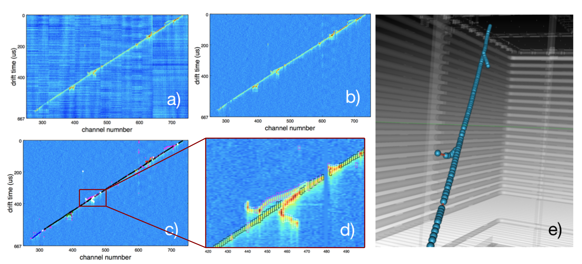
\includegraphics[width=\textwidth,keepaspectratio]{event_larsoft.png}
          \caption[Reconstruction d'un événement dans LArSoft]{\label{fig::event_larsoft}Reconstruction d'un événement dans \gls{larsoft}. a) données après suppression du piédestal, b) après suppression du bruit, c) identification des hits, d) groupement en amas, e) reconstruction 3D de la trace.}
        \end{figure}
        Les données brutes enregistrées par l'électronique du \TOO{} sont des fichiers binaires, contenant l'information de la tension mesurée (en ADC) pour les \numprint{1667} bin de temps de \SI{0.4}{\micro\second} de chacun des \numprint{1280} canaux de lecture (\numprint{320} en vue 0 et \numprint{960} en vue 1). Le logiciel \gls{larsoft}\footnote{\url{http://larsoft.org}} a été utilisé pour reconstruire les événements. Il s'agit d'un logiciel C++ utilisant ROOT dédié à l'étude de toutes les \gls{lartpc} existantes ou prévues, \protodp{} inclue.  La reconstruction, illustrée par la \autoref{fig::event_larsoft}, se fait selon les étapes suivantes :
        \begin{enumerate}
          \item Identification des \gls{roi} : zone où il y a probablement des coups.
          \item Soustraction du piédestal et aplatissement du signal grâce à un ajustement polynomial.
          \item Soustraction du bruit cohérent et du bruit périodique.
          \item Identification des coups et mesure du dépôt de charge $dQ$.
          \item Regroupement des coups en amas à deux dimensions.
          \item Identification des amas à trois dimensions : quel amas en vue 0 correspond à quel amas en vue 1?
          \item Reconstruction de la trace en trois dimensions et calcul de la longueur de déposition de charge $ds$ pour chaque coup.
        \end{enumerate}
        L'identification des régions d'intérêt se fait canal par canal avec un simple  système de seuil. Toute région au dessus d'une limite d'ADC et vue comme potentiel coup. Un polynôme est ensuite ajusté sur le canal, en ignorant les \gls{roi}, afin de soustraire le piédestal et de corriger d'éventuelle fluctuations lentes du signal vu par le canal. Les bruits présentant un signal périodique sont soustraits grâce à des transformations de Fourier. Le bruit cohérent, identique parmi les 32 canaux regroupés sur chaque carte électronique, est soustrait en moyennant sur chaque groupe de 32 canaux l'ADC vu dans chaque bin de temps, \gls{roi} exclus. Ceci est répété plusieurs fois, de nouvelles \gls{roi} pouvant apparaître. Les coups sont ensuite identifiés par un seuil en ADC, dans chaque vue séparément. Ces coups sont regroupés en amas à deux dimensions. La première dimension est selon le temps d'arrivée, correspondant à la hauteur du détecteur, l'autre est soit le largeur (vue 0) soit la longueur (vue 1). Les amas dans une vue sont ensuite identifiés aux amas dans l'autre vue afin de reconstruire une trace en trois dimension, nécessaire pour calculer la longueur de déposition de charge $ds$. Le calcul de $ds$ entre deux coups consécutif est illustré en \autoref{fig::ds-schema}. Une fois cela fait, l'information $dQ/ds$ est disponible pour chaque coup.

        \begin{figure}[htbp]
          \centering
          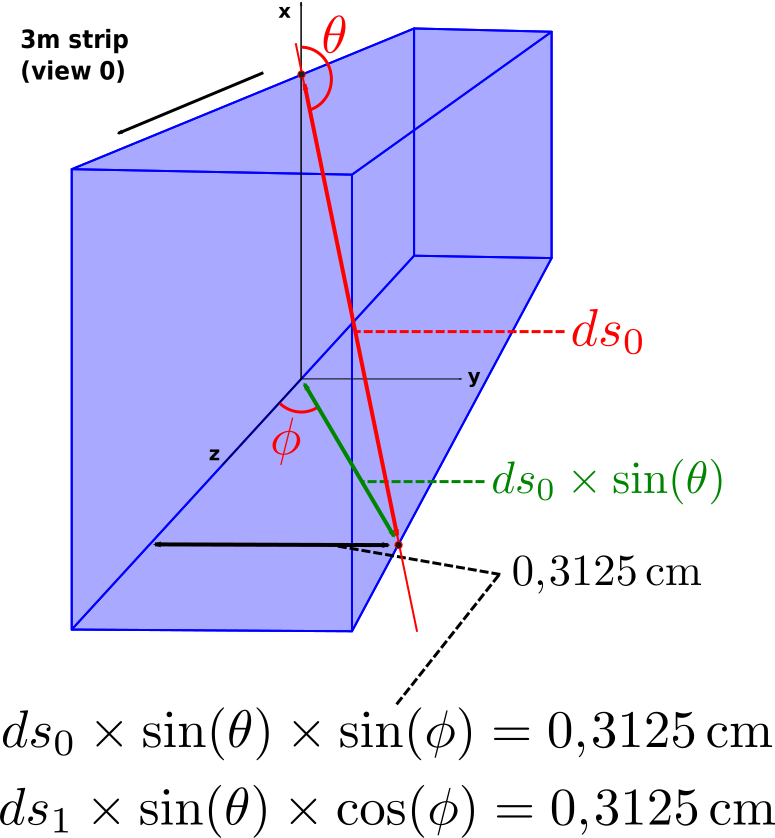
\includegraphics[width=0.65\textwidth,keepaspectratio]{ds.pdf}
          \caption[Schéma du calcul de $ds$]{\label{fig::ds-schema}Schéma du calcul de $ds$ entre deux coups consécutifs (points oranges). Le segment rouge représente la trace de la particule traversant un élément de volume délimité par la largeur d'un canal de lecture en vue 0, $ds_0$ désigne $ds$ en vue 0 et $ds_1$ désigne $ds$ en vue 1.}
        \end{figure}

      \subsubsection{Sélections des muons}\label{sec::selection}

        \begin{figure}[htbp]
          \centering
          \includegraphics[width=\textwidth,keepaspectratio]{highway.png}
          \caption[Illustration de l'algorithme de sélection des muons]{\label{fig::highway}Illustration de l'algorithme de sélection des muons. Le ratio entre la charge totale déposée dans la zone orange et celle déposée dans la zone verte doit être faible pour une trace de muon, qui ne fait pas de gerbe et n'est pas dévié durant la traversée du détecteur.}
        \end{figure}

        Pour l'analyse du gain présentée ici, seul les muons devaient être utilisés, la \gls{mpv} de la distribution $dQ/ds$ attendue étant connue. Un algorithme capable d'identifier ces derniers a été développé au CERN. Il se base sur le fait qu'un muon cosmique traversant le détecteur aura une trace unique, droite et étroite, contrairement à une gerbe électromagnétique ou hadronique. En regardant la distribution de la charge autour des traces reconstruites, il est possible de définir un critère de sélection des muons. La \autoref{fig::highway} illustre le fonctionnement de cet algorithme : les traces sont segmenté en morceaux de \SI{50}{\centi\meter} et deux régions sont définies autour de chaque segment. Une grande région "A" et petit région "B" (inclue dans la grande région). Les sommes des charges déposée dans ces région, $Q_A$ et $Q_B$, sont calculées et le critère pour sélectionner un muon est le suivant :
        \begin{equation}\label{eq::cbr}
          \frac{Q_A-Q_B}{Q_A} < 0.1
        \end{equation}
        En effet, si la trace est un muon, la grande majorité de la charge sera dans la petite région, les charges $Q_A$ et $Q_B$ sont alors presque identiques. La dimension et le positionnement autour de la trace de ces régions dépendra de l'angle de la trace. En effet, on peut le voir en \autoref{fig::highway}, une "traînée" est observable en bas de la trace à cause de l'extraction des électrons qui étale le signal en temps. Une trace horizontale aura une traînée perpendiculaire à sa trajectoire et la charge sera vue dans une région plus grande que pour une trace presque verticale. Les régions doivent alors être plus grande.

        En plus de cet algorithme, des coupures sont mises sur la longueur et sur les angles des traces (les traces parallèles aux canaux d'une vue sont plus difficiles à reconstruire). L'efficacité de ces sélections a été étudiée par les collaborateurs au \gls{cern} sur une simulation Monte-Carlo du détecteur, réalisée avec GEANT4 et CORSIKA. Après sélection, sont conservés \numprint{68.2}\,\% des événements issu de muons primaires, \numprint{6.29}\,\% de pions primaires et \numprint{0.35}\,\% d'électrons primaires. Au total, \numprint{17}\,\% des traces sont conservées avec \numprint{92}\,\% de muons.

        Une coupure supplémentaire consiste à ne sélectionner que les traces qui traversent entièrement le détecteur de bas en haut. En effet, pour une telle trace, il n'y a pas d'ambiguïté quant à la position des coups le long de la hauteur du détecteur : les coups au premier bin de temps sont au niveau du \gls{crp} tandis que les coups au dernier bin de temps sont en bas du détecteur (la durée d'enregistrement d'un événement est de \SI{667}{\micro\second}, soit \SI{1.09}{\meter} à une vitesse de dérive de \SI{1.63}{\milli\meter\per\micro\second}). Dans ce cas là, il est possible d'estimer le pourcentage de charge perdu à cause des impuretés et de corriger le $dQ$ mesuré. En revanche, si une trace commence ou fini au milieu du détecteur, cela peut signifier qu'une particule est arrivée dans le volume fiduciel alors que l'enregistrement de l'événement avait déjà commencé (ou inversement, qu'elle était déjà là). il est alors impossible de savoir depuis combien de temps les électrons de ces traces dérivent et la correction pour les pertes dues aux impuretés ne peut pas être prise en compte.

        A noter que due à la faible quantité de données collectée dans le \TOO{}, la pureté n'a pas pu être mesurée. Une valeur de $\tau_e = \SI{7}{\milli\second}$ pour le temps de vie des électrons a été utilisée, correspondant à la pureté achevée dans \protosp{}.
        
      \subsubsection{Corrections et normalisations aux données du \threeL{}}
        
        Afin de pouvoir comparer les mesures du \TOO{} à celles effectuées en 2014 dans le prototype de \threeL{}, plusieurs normalisations doivent être appliquées. De plus, des corrections doivent être appliquées à chaque coup mesuré.

        \paragraph{Correction : pureté :} Comme mentionné dans la section précédente, un temps de vie des électrons dans l'argon liquide de $\SI{7}{\milli\second}$ a été utilisé pour prendre en compte les pertes dues aux impuretés. Cette correction est appliquée à chaque coup séparément. La perte due aux impuretés est, au maximum, de 8\,\%.

        \paragraph{Correction : charging up :} Le gain effectif va diminuer au cours du temps due à la présence des RIMs autour des trous d'amplification des \glspl{lem}. Dans chaque run de prise de données de plus d'une heure, cette diminution est visible et peut être prise en compte pour le calculer de la \gls{mpv}. Plus de détail en \autoref{sec::res-stab-cu}.

        \paragraph{Correction : distance de dépôt de charge:} La \gls{mpv} de la Landau-Vavilov est donnée par l'équation \eqref{eq::mpv}, qui croît logarithmiquement avec $ds$, la distance de dépôt de charge. La dépendance de la \gls{mpv} à $ds$ peut induire des variations de \gls{mpv} allant jusqu'à 10\,\% (voir \autoref{fig::mpv_ds}). Tous les coups ont été corrigés pour cet effet, en multipliant le $dQ/ds$ mesuré par le ratio $MPV_{ds=\SI{1}{\centi\meter}}/MPV_{ds}$. La valeur de $ds=\SI{1}{\centi\meter}$ a été choisie comme référence car c'est la valeur la plus souvent mesurée dans le prototype (voir \autoref{fig::ds_840_842}).

        \paragraph{Normalisation : efficacité d'extraction et de collection:} Les champs d'extraction et d'induction ont une influence sur l'efficacité d'extraction et de collection des charges à travers le \gls{crp}. Les éventuelles pertes d'électrons sont prises en compte dans le facteur $\mathcal{T}$ du gain effectif (voir \autoref{eq::gain_eff}). Dans le \TOO{}, ces champs variaient d'un run à l'autre, et étaient inférieurs aux champs nominaux utilisés par le \threeL{}. Un facteur correctif doit alors êtres appliqué pour se ramener aux valeurs du champs du \threeL{} afin de regarder la variation du gain en fonction du champ d'amplification. Ce facteur est calculé grâce aux simulations présentées en \autoref{sec::efficacites} et aux études de l'efficacité d'extraction réalisées par Gushchin et.al en 1982\cite{guschin} (voir \autoref{sec::extraction}). Afin d'estimer le champ dans le gaz ainsi que le champ dans le liquide, la formule \eqref{eq::fields_liquid_gas} est utilisée, qui prend en compte la position de l'interface liquide-gaz entre la grille d'extraction et les \glspl{lem}. En effet, nous en parlons plus loin, cette interface se trouvait en moyenne à \SI{7}{\milli\meter} au dessus de la grille et non pas à \SI{5}{\milli\meter}.

        \paragraph{Normalisation : densité:} Les mesures du \threeL{} ont été faites à une pression de \SI{980}{\milli\bar} et à une température au niveau des \glspl{lem} de \SI{87}{\kelvin}. Dans le \TOO{}, la pression moyenne était de \SI{999}{\milli\bar} et la température au niveau des \glspl{lem} de \SI{89}{\kelvin} (voir \autoref{sec::slow_control}). En ajustant l'équation du gain effectif \eqref{eq::gain_eff} aux données du \threeL{}, il est possible de calculer le gain attendu à la densité dans le \TOO{} et d'appliquer un facteur correctif aux $dQ$ mesurés.

    \subsection{Principales incertitudes}\label{sec::uncertainties}
        
      \begin{figure}[htbp]
        \centering
        \includegraphics[width=\textwidth,keepaspectratio]{CRP-metrologie.png}
        \caption[Mesure de la planéité du CRP]{\label{fig::crp_var}Mesure de la planéité du \gls{crp} par photogrammétrie. Le zéro correspond à une distance entre la grille est le \gls{lem} de \SI{10}{\milli\meter}.}
      \end{figure}

      \begin{figure}[htbp]
        \centering
        \begin{subfigure}[t]{0.48\textwidth}
          \centering
          \includegraphics[width=\textwidth,keepaspectratio]{thickness.pdf}
          \caption[Mesures d'épaisseur des LEMs du \TOO{}]{\label{fig::lem_thicnkess_311}Mesures d'épaisseur des \glspl{lem} du \TOO{}, décrites dans le papier technique de 2018\cite{Aimard2018}.}
        \end{subfigure}\hfill
        \begin{subfigure}[t]{0.48\textwidth}
          \centering
          \includegraphics[width=\textwidth,keepaspectratio]{capa.pdf}
          \caption[Capacitance moyenne entre la grille d'extraction et les LEMs en fonction du niveau de l'interface liquide-gaz]{\label{fig::capa}Capacitance moyenne entre la grille d'extraction et les \glspl{lem} en fonction du niveau de l'interface liquide-gaz, ajusté par un modèle de capacité à deux plaques parallèles.}
%            \centering
%            \includegraphics[width=\textwidth,keepaspectratio]{gain_var_dg.pdf}
%            \caption[Variation du gain en fonction de la variation de la distance interface-\gls{lem}]{\label{fig::systematiques_dg}Variation du gain en fonction de la variation de la distance interface-\gls{lem}, prenant en compte le gradient de température dans le gaz et les efficacités d'extraction et de collection, qui dépendent des champs électriques dans le liquide et le gaz.}
        \end{subfigure}
      \end{figure}


      \begin{figure}[htbp]
        \centering
        \begin{subfigure}[t]{0.48\textwidth}
          \centering
          \includegraphics[width=\textwidth,keepaspectratio]{fields_vs_dg_gas.pdf}
          \caption{Variations du champ dans le gaz dues aux déformation du \gls{crp} pour plusieurs valeur de tension d'extraction.}
        \end{subfigure}\hfill
        \begin{subfigure}[t]{0.48\textwidth}
          \centering
          \includegraphics[width=\textwidth,keepaspectratio]{fields_vs_dg_liquid.pdf}
          \caption{Variations du champ dans le liquide dues aux déformation du \gls{crp} pour plusieurs valeur de tension d'extraction.}
        \end{subfigure}
        \caption[Variations des champs d'extraction dues à la déformation du CRP]{\label{fig::fields_vs_dg}Variations des champ dans le liquide et le gaz entre la grille et les \glspl{lem} dues aux déformation du \gls{crp} pour plusieurs valeur de tension d'extraction.}
      \end{figure}

      \begin{figure}[htbp]
        \centering
        \includegraphics[width=0.8\textwidth,keepaspectratio]{eff_guschin_and_combined.pdf}
        \caption[Efficacité combinée d'extraction et de collection en fonction du champ dans le liquide]{\label{fig::eff_guschin_and_combined}Variation de l'efficacité d'extraction (triangles rouges pleins) et de l'efficacité combinée d'extraction et de collection du \gls{lem} en fonction du champ dans le liquide, en supposant une distance grille-interface de \SI{7}{\milli\meter} et une distance interface-\glspl{lem} de \SI{2}{\milli\meter}.}
      \end{figure}

      Le gain dans une \gls{lartpc} est influencé fortement par l'épaisseur des \glspl{lem}, comme nous l'avons discuté en \autoref{sec::epaisseur}. La densité du gaz, qui apparaît dans l'équation de l'avalanche de Townsed \eqref{eq::townsend} aux mêmes endroits que l'épaisseur, aura la même influence. La \autoref{fig::lem_thicnkess_311} présente les mesures d'épaisseur réalisées au \gls{cern} sur les \glspl{lem} présents dans le \TOO{}, dont l'impact sur le gain sera de la dizaine de pourcent. La densité est proportionnelle au rapport de la pression et de la température, deux grandeurs stables au cours du temps dans le \TOO{} (voir \autoref{sec::slow_control}) dont les petites variations auront un impact de l'ordre du pourcent sur le gain. 

      La température, stable au cours du temps, va cependant varier en fonction de la distance avec l'interface liquide-gaz. Or des mesures de photogrammétrie ont été réalisées sur le \gls{crp} et ont révélé que la distance entre la grille est les \glspl{lem} variait entre \SI{7.2}{\milli\meter} et \SI{10.8}{\milli\meter}, comme le montre la \autoref{fig::crp_var}. Ces mesures ont été faites à froid, mais avant insertion du \gls{crp} dans le cryostat. Il n'est donc pas possible de savoir quelle région du \gls{crp} présentait quelle variation durant les opérations. Afin d'estimer l'impact de ces déformations sur le gain, il a été supposé que la distance grille-\gls{lem} suivait une distribution uniforme entre \SI{7.2}{\milli\meter} et \SI{10.8}{\milli\meter}. Le gradient de température a été mesuré grâce à des capteurs placés sur le cryostat (voir \autoref{sec::slow_control}) afin d'estimer les variations de températures. Les variations relatives calculée sont dix fois plus faibles que les variations relatives de l'épaisseur, et sont donc négligeables face à ces dernières.

      La déformation du \gls{crp} va également jouer un rôle sur les champs électriques dans le gaz et dans le liquide entre la grille et les \glspl{lem}. Ces champs électriques vont à leur tour avoir une influence sur l'efficacité d'extraction liquide-gaz, discuté en \autoref{sec::extraction} et sur l'efficacité de collection du \gls{lem}, discuté en \autoref{sec::efficacites}, dans cette même région. Afin d'évaluer ces champs, il faut connaître la distance entre la grille et l'interface ainsi que la distance entre l'interface et les \glspl{lem}. Aucune déformation significative n'a été observée, et le niveau d'argon liquide était très stable durant toute la duré des prises de données (voir \autoref{sec::slow_control}). La distance grille-interface était donc considérée comme constante. Une mesure de capacitance entre les \glspl{lem} et la grille (voir \autoref{fig::capa}) a permit d'estimer cette valeur à \SI{7}{\milli\meter} durant les opérations. La moyenne des capacitances de chaque \gls{lem} était calculée tout en faisant augmenter le niveau d'argon liquide, mesuré avec un des capteur de niveau installé sur le bord du \gls{crp}. En ajustant sur ces mesures un modèle de capacité à deux plaques parallèles, il est possible de connaître la capacitance en fonction du niveau. Les variations des champs électriques sont alors calculables avec la formule \eqref{eq::fields_liquid_gas}. Elles sont présentées en fonction de la distance interface-\glspl{lem} en \autoref{fig::fields_vs_dg} pour les valeurs de tension d'extraction utilisées dans le \TOO{}.

      La \autoref{fig::eff_guschin_and_combined} montre l'influence du champ dans le liquide sur l'efficacité d'extraction (triangles rouges pleins) ainsi que sur l'efficacité combinée d'extraction et de collection du \gls{lem} (triangles oranges vides), en supposant une distance interface-\glspl{lem} fixée à \SI{2}{\milli\meter}. On constate qu'une augmentation de champ de \numprint{1.25} à \SI{1.75}{\kilo\volt\per\centi\meter} entraîne une augmentation de l'efficacité combinée de près de 40\,\%. Donc, à basse tension d'extraction, les variations de champ induites par la déformation du \gls{crp} auront une grande influence sur l'efficacité combinée, alors qu'à plus haute tension, où l'efficacité combinée atteint un plateau, les déformations auront peu d'effet.

      Il est important de noter que la valeur de \SI{7}{\milli\meter} pour la distance grille-interface ainsi que l'intervalle \numprint{7.2}--\SI{10.8}{\milli\meter} pour la distance grille \glspl{lem} ne sont pas connus avec une grande précision. Ces valeurs sont utilisées fautes de mieux et aucunes incertitudes ne leur sont associées. De même, aucune incertitude n'est associée aux efficacités d'extraction et de collection.

      Dans le \TOO{}, les différents runs ont été pris à des tensions d'extraction différentes, et l'impact de la déformation du \gls{crp} sur le gain effectif a été calculé et combiné à l'impact de la variation d'épaisseur des \glspl{lem} pour produire les barres d'erreurs présentes sur les différents graphiques qui suivent.

      Les grilles d'extraction des \glspl{crp} du \SSS{} ont atteint la tension nominale dans la boîte cryogénique. Les champs dans le liquide et le gaz seront alors stables même si les \glspl{crp} présentent des déformation de l'ordre du \si{\milli\meter}, et l'incertitude principale viendra de l'épaisseur des \glspl{lem} dont l'effet sur le gain est montrée en \autoref{fig::exp_gain_range}.
    
%        Les incertitudes liées à la variation de la \gls{mpv} attendue due à l'ignorance de l'impulsion des muons initiales a été négligée. La \gls{mpv} étant un minimum local, ses variations sont faibles. Les incertitudes liées aux variations dans le temps de la pression et température, présentées en \autoref{sec::slow_control}, sont estimées autour de 1\,\% et sont également négligées. Les variations dues aux imprécisions de mesures sur $dQ$ et $ds$ sont négligées.
        
  \section{Données collectées}\label{sec::data-311}

    La collection des données s'est faite entre Juin et Novembre 2017. Des problèmes de tenue en tension ont empêché l'opération aux champs nominaux recommandés par les études du \threeL{} : la grille d'extraction n'a pas atteint les tensions nominales. Ceci a limité les valeurs possibles de champs d'amplification, d'induction et d'extraction : augmenter un de ces champs impliquait de diminuer le maximum sur un autre. De plus, des décharges arrivaient régulièrement, et donc les runs n'excèdent pas quelques heures. Prendre des données à un champ d'amplification supérieur à \SI{28}{\kilo\volt\per\centi\meter} impliquait un potentiel entre la grille est les \glspl{lem} autour de \SI{1}{\kilo\volt}. À cette tension, l'extraction est lente et un grand nombre d'électrons sont perdus, produisant des runs difficiles à analyser. Plus de détails sont apportés en \autoref{sec::results-311}.
 
    \subsection{Champs scannés}

      
    \nonstopmode
    \begin{longtable}{|l||cccccccc|}
      \caption[Données collectées dans le \TOO{}.]{\label{tab::data-collected}Données collectées dans le \TOO{} entre Juin et Novembre 2017. Les champs électriques sont en \si{\kilo\volt\per\centi\meter}, les \gls{mpv} en \si{\femto\coulomb\per\centi\meter}. Les runs en verts sont utilisés pour le scan d'extraction, les runs en bleu ainsi que les run 840 et 842 sont utilisés pour le scan en amplification. Ces derniers, en rouge, sont également utilisés pour analyser le charging up et la stabilité du gain sur la surface du \gls{crp}.}
\\    \hline
         Run & Date & Durée & traces(coups) & $E_{LEM}$ & $E_{ind}$ & $E_{extr-g(l)}$ &  $\frac{MPV_0}{MPV_1}$ & $G_{eff}$ \\
      \hline
      \endhead
      \endfoot
        \textcolor{green}{785} & 19/07 & 09\,min & 55(\numprint{1.8}\,k) & \numprint{28} & \numprint{1} & \numprint{2.3}(\numprint{1.5}) & \numprint{1.1} & \numprint{1.3} \\
        \textcolor{green}{786} & 19/07 & 08\,min & 90(\numprint{4.3}\,k) & \numprint{28} & \numprint{1} & \numprint{2.4}(\numprint{1.6}) & \numprint{0.99} & \numprint{1.2} \\
        \textcolor{green}{787} & 19/07 & 08\,min & 69(\numprint{3.7}\,k) & \numprint{28} & \numprint{1} & \numprint{2.6}(\numprint{1.7}) & \numprint{1.1} & \numprint{1.3} \\
        \textcolor{green}{788} & 19/07 & 08\,min & 114(\numprint{7.7}\,k) & \numprint{28} & \numprint{1} & \numprint{2.7}(\numprint{1.8}) & \numprint{1} & \numprint{1.3} \\
        \textcolor{green}{789} & 19/07 & 09\,min & 168(\numprint{14}\,k) & \numprint{28} & \numprint{1} & \numprint{2.9}(\numprint{1.9}) & \numprint{1.1} & \numprint{1.4} \\
        \textcolor{green}{790} & 19/07 & 08\,min & 176(\numprint{14}\,k) & \numprint{28} & \numprint{1} & \numprint{3}(\numprint{2}) & \numprint{1.1} & \numprint{1.4} \\
        \textcolor{green}{791} & 19/07 & 08\,min & 163(\numprint{16}\,k) & \numprint{28} & \numprint{1} & \numprint{3.2}(\numprint{2.1}) & \numprint{1.1} & \numprint{1.4} \\
        \textcolor{green}{792} & 19/07 & 08\,min & 191(\numprint{20}\,k) & \numprint{28} & \numprint{1} & \numprint{3.3}(\numprint{2.2}) & \numprint{1.1} & \numprint{1.5} \\
        \textcolor{green}{793} & 19/07 & 09\,min & 205(\numprint{20}\,k) & \numprint{28} & \numprint{1} & \numprint{3.5}(\numprint{2.3}) & \numprint{1} & \numprint{1.5} \\
        \textcolor{green}{794} & 19/07 & 08\,min & 183(\numprint{21}\,k) & \numprint{28} & \numprint{1} & \numprint{3.6}(\numprint{2.4}) & \numprint{1.1} & \numprint{1.5} \\
        \textcolor{green}{795} & 19/07 & 08\,min & 146(\numprint{16}\,k) & \numprint{28} & \numprint{1} & \numprint{3.8}(\numprint{2.5}) & \numprint{1} & \numprint{1.5} \\
        \textcolor{green}{796} & 19/07 & 02\,min & 22(\numprint{1.5}\,k) & \numprint{28} & \numprint{1} & \numprint{3.9}(\numprint{2.6}) & \numprint{0.96} & \numprint{1.4} \\
        \textcolor{red}{840} & 26/07 & 10\,h\,06\,min & 156(\numprint{6.9}\,k) & \numprint{28} & \numprint{1.5} & \numprint{2.9}(\numprint{1.9}) & \numprint{0.94} & \numprint{1.8} \\
        \textcolor{red}{842} & 27/07 & 4\,h\,10\,min & 85(\numprint{4.6}\,k) & \numprint{28} & \numprint{1.5} & \numprint{2.9}(\numprint{1.9}) & \numprint{0.95} & \numprint{1.7} \\
        \textcolor{blue}{988} & 29/08 & 4\,h\,09\,min & 30(\numprint{1.4}\,k) & \numprint{25} & \numprint{1} & \numprint{3.3}(\numprint{2.2}) & \numprint{0.86} & \numprint{0.56} \\
        \textcolor{blue}{993} & 30/08 & 14\,h\,01\,min & 101(\numprint{5.8}\,k) & \numprint{26} & \numprint{1} & \numprint{3.3}(\numprint{2.2}) & \numprint{0.9} & \numprint{0.67} \\
        \textcolor{blue}{996} & 31/08 & 4\,h\,59\,min & 63(\numprint{3.8}\,k) & \numprint{26} & \numprint{1} & \numprint{3.3}(\numprint{2.2}) & \numprint{1.2} & \numprint{0.59} \\
        \textcolor{blue}{998} & 31/08 & 9\,h\,03\,min & 111(\numprint{6.4}\,k) & \numprint{26} & \numprint{1} & \numprint{3.3}(\numprint{2.2}) & \numprint{0.93} & \numprint{0.8} \\
        \textcolor{blue}{1002} & 01/09 & 3\,h\,18\,min & 30(\numprint{1.3}\,k) & \numprint{27} & \numprint{1} & \numprint{3.2}(\numprint{2.1}) & \numprint{0.94} & \numprint{0.94} \\
        \textcolor{blue}{1036} & 06/09 & 6\,h\,46\,min & 34(\numprint{1.1}\,k) & \numprint{28} & \numprint{1.2} & \numprint{3}(\numprint{2}) & \numprint{0.96} & \numprint{1.1} \\
        \textcolor{blue}{1197} & 10/11 & 30\,min & 1(\numprint{0}\,k) & \numprint{30} & \numprint{2} & \numprint{1.5}(\numprint{1}) & \numprint{1} & \numprint{3.5} \\
        \textcolor{blue}{1199} & 10/11 & 33\,min & 3(\numprint{0.1}\,k) & \numprint{31} & \numprint{1} & \numprint{1.7}(\numprint{1.1}) & \numprint{0.99} & \numprint{3} \\
        \threeL{} & 2013 &  &  & \numprint{28.5}--35 & \numprint{5} & \numprint{3}(\numprint{2}) &  &  \\
      \hline
    \end{longtable}


          \begin{table}
      \centering
      \begin{tabular}{|l||ccccccccc|}
      \hline
         Run & $G_{corr}$ & $3L_{b.c.u}$ & $3L_{a.c.u}$ & $Eff_{extr}(3L)$ & $Eff_{LEM}(3L)$ & $Eff_{Anode}(3L)$ & $\rho_{corr}$ & $\frac{3L_{b.c.u}}{G_{311}}$ & $\frac{3L_{a.c.u}}{G_{311}}$ \\
      \hline
       840 & \numprint{3.2} & \numprint{6} & \numprint{3.2} & \numprint{0.71}(\numprint{0.85}) & \numprint{0.73}(\numprint{0.67}) & \numprint{0.33}(\numprint{0.58}) & \numprint{0.93} & \numprint{1.8} & \numprint{0.97} \\
        842 & \numprint{3.1} & \numprint{6} & \numprint{3.2} & \numprint{0.71}(\numprint{0.85}) & \numprint{0.73}(\numprint{0.67}) & \numprint{0.33}(\numprint{0.58}) & \numprint{0.93} & \numprint{1.9} & \numprint{1} \\
        988 & \numprint{1.2} & \numprint{2.6} & \numprint{1.6} & \numprint{0.82}(\numprint{0.85}) & \numprint{0.66}(\numprint{0.65}) & \numprint{0.26}(\numprint{0.56}) & \numprint{0.93} & \numprint{2.2} & \numprint{1.4} \\
        993 & \numprint{1.4} & \numprint{2.9} & \numprint{1.8} & \numprint{0.82}(\numprint{0.85}) & \numprint{0.66}(\numprint{0.65}) & \numprint{0.26}(\numprint{0.56}) & \numprint{0.93} & \numprint{2.1} & \numprint{1.3} \\
        996 & \numprint{1.3} & \numprint{3.3} & \numprint{2} & \numprint{0.82}(\numprint{0.85}) & \numprint{0.66}(\numprint{0.66}) & \numprint{0.26}(\numprint{0.56}) & \numprint{0.93} & \numprint{2.6} & \numprint{1.6} \\
        998 & \numprint{1.8} & \numprint{3.8} & \numprint{2.2} & \numprint{0.82}(\numprint{0.85}) & \numprint{0.67}(\numprint{0.66}) & \numprint{0.25}(\numprint{0.57}) & \numprint{0.93} & \numprint{2.1} & \numprint{1.2} \\
        1002 & \numprint{2.2} & \numprint{4.4} & \numprint{2.4} & \numprint{0.8}(\numprint{0.85}) & \numprint{0.68}(\numprint{0.67}) & \numprint{0.24}(\numprint{0.58}) & \numprint{0.93} & \numprint{2} & \numprint{1.1} \\
        1036 & \numprint{2.3} & \numprint{5.1} & \numprint{2.8} & \numprint{0.75}(\numprint{0.85}) & \numprint{0.72}(\numprint{0.67}) & \numprint{0.29}(\numprint{0.58}) & \numprint{0.93} & \numprint{2.2} & \numprint{1.2} \\
        1197 & \numprint{11} & \numprint{13} & \numprint{6} & \numprint{0.3}(\numprint{0.85}) & \numprint{0.94}(\numprint{0.7}) & \numprint{0.38}(\numprint{0.59}) & \numprint{0.93} & \numprint{1.2} & \numprint{0.56} \\
        1199 & \numprint{12} & \numprint{20} & \numprint{8.8} & \numprint{0.35}(\numprint{0.85}) & \numprint{0.91}(\numprint{0.71}) & \numprint{0.26}(\numprint{0.58}) & \numprint{0.93} & \numprint{1.7} & \numprint{0.74} \\
      \hline
      \end{tabular}
      \caption[Données collectées dans le \TOO{} normalisées aux conditions d'opération du \threeL{}]{\label{tab::data-3L}Données collectées dans le \TOO{} normalisées aux conditions d'opération du \threeL{}. $G_{corr}$ est le gain dans le \TOO{} ramené au valeurs de champs et de densité du \threeL{}. Les abréviations $a.c.u$ et $b.c.u$ signifient respectivement \textit{after charging up} et \textit{before charging up}. Pour les colonnes $Eff_{extr}$, $Eff_{LEM}$ et $Eff_{Anode}$ la première valeur est celle dans le \TOO{}, la valeur entre parenthèses est celle dans le \threeL{}.}
    \end{table}

      Afin d'étudier le comportement du gain en fonction du champ d'extraction, 12 runs ont été pris à champ d'amplification et champ d'induction constants, et en faisant varier le potentiel entre la grille et les \glspl{lem} de \SI{1.5}{\kilo\volt} à \SI{2.6}{\kilo\volt}. Due a des problèmes de tenus en tension, ce potentiel était limité, réduisant les possibilités de réaliser un scan en amplification à champ d'extraction constant. Ce scan a été réalisé en faisant varier le champ d'extraction et le champ d'induction, et les données sont alors corrigées pour les variations d'efficacités d'extraction et de collection. Pour les mêmes raisons de tenu en tension, un scan selon l'induction n'a pas pu être réalisé. Le \autoref{tab::data-collected} présente la liste des runs utilisés pour les différents scans. Le \autoref{tab::data-3L} présente, pour les runs du scan d'amplification, la normalisation aux données du \threeL{}. Deux runs, les 840 et 842, stables sur plusieurs heures, ont été utilisés pour les analyses du charging up et de l'uniformité du gain sur le \gls{crp}. Ils sont en rouge dans le \autoref{tab::data-collected}.

      Les runs utilisés pour le scan en extraction étant particulièrement courts, ne sélectionner que les traces traversant entièrement le détecteur ne laissait pas assez de coups pour mesurer les \glspl{mpv}. Cette coupure est donc ignorée, expliquant le nombre de traces  important de ces runs par rapport à leur durée. La correction pour la pureté n'était alors pas appliquée.

    \subsection{Slow control}\label{sec::slow_control}

      \begin{figure}[htbp]
        \centering
        \includegraphics[width=\textwidth,keepaspectratio]{slow_control.png}
        \caption[Variation de température et de niveau d'argon dans le \TOO{}]{\label{fig::slow_control}Variation de température (droite) et de niveau d'argon (gauche) dans le \TOO{} durant une semaine. Les graphiques viennent du TDR de 2018\cite{Aimard2018}.}
      \end{figure}

      \begin{figure}[htbp]
        \centering
        \begin{subfigure}[t]{0.48\textwidth}
          \centering
          \includegraphics[width=\textwidth,keepaspectratio]{pressure.pdf}
          \caption[Pression dans le \TOO{} au cours du run 840]{\label{fig::pressure}Pression dans le \TOO{} au cours du run 840.}
        \end{subfigure}\hfill
        \begin{subfigure}[t]{0.48\textwidth}
          \centering
          \includegraphics[width=\textwidth,keepaspectratio]{temp_vs_height.pdf}
          \caption[Gradient de température dans le \TOO{} durant le run 840]{\label{fig::temp_vs_height}Gradient de température dans le \TOO{} durant le run 840. La partie constante correspond aux capteur dans le liquide, la partie linéairement croissante correspond à ceux dans le gaz.}
        \end{subfigure}
      \end{figure}
      
%      LAr level stability: 100 microns
%• precision of monitoring: 100 microns
%• absolute positioning of the frame with 3 point suspension system:100 microns
      Durant les opérations du \TOO{}, la température, la pression et le niveau d'argon étaient surveillés en direct par un dispositif de slow control. La \autoref{fig::slow_control} montre l'évolution au cours du temps de 4 capteurs de température, placés à des heuteurs différentes dans la phase gazeuse, et d'un capteur de niveau sur une période d'une semaine. La \autoref{fig::pressure} montre les variation de la pression durant le run 840. Le niveau de l'interface liquide-gaz est très stable, et aucune correction n'est nécessaire. La température baisse légèrement sur une semaine, mais peut être considéré comme constante durant un même run. Les variations de température entre les runs ont été prises en compte à travers la correction de densité discutée précédemment : pour chaque run, la température moyenne été calculée pour chaque capteurs de température, et un ajustement linéaire de la température en fonction de la position du capteur selon la hauteur permettait de mesurer le gradient dans le gaz et ainsi d'estimer la température à \SI{2.5}{\milli\meter} au dessus du niveau du liquide, qui est la position moyenne du milieu du \gls{lem}. La \autoref{fig::temp_vs_height} montre cet ajustement pour le run 840. La pression moyenne pour chaque run a également été prise en compte dans cette correction.

  \section{Résultats}\label{sec::results-311}

    \subsection{Distributions $dQ/ds$ et $ds$}

      \begin{figure}[htbp]
        \centering
        \begin{subfigure}[t]{0.48\textwidth}
          \centering
          \includegraphics[width=\textwidth,keepaspectratio]{dQds_840_0.pdf}
          \caption{Vue 0, run 840.}
        \end{subfigure}\hfill
        \begin{subfigure}[t]{0.48\textwidth}
          \centering
          \includegraphics[width=\textwidth,keepaspectratio]{dQds_840_1.pdf}
           \caption{Vue 1, run 840.}
        \end{subfigure}\\
        \begin{subfigure}[t]{0.48\textwidth}
          \centering
          \includegraphics[width=\textwidth,keepaspectratio]{dQds_842_0.pdf}
          \caption{Vue 0, run 842.}
        \end{subfigure}\hfill
        \begin{subfigure}[t]{0.48\textwidth}
          \centering
          \includegraphics[width=\textwidth,keepaspectratio]{dQds_842_1.pdf}
          \caption{Vue 1, run 842.}
        \end{subfigure}
        \caption[Distribution de la charge déposée par unité de longueur dans le \TOO{}]{\label{fig::dqds_840_842}Distribution de la charge déposée par unité de longueur dans le \TOO{}.}
      \end{figure}

      \begin{figure}[htbp]
        \centering
        \begin{subfigure}[t]{0.48\textwidth}
          \centering
          \includegraphics[width=\textwidth,keepaspectratio]{ds_840_0.pdf}
          \caption{Vue 0, run 840.}
        \end{subfigure}\hfill
        \begin{subfigure}[t]{0.48\textwidth}
          \centering
          \includegraphics[width=\textwidth,keepaspectratio]{ds_840_1.pdf}
          \caption{Vue 1, run 840.}
        \end{subfigure}\\
        \begin{subfigure}[t]{0.48\textwidth}
          \centering
          \includegraphics[width=\textwidth,keepaspectratio]{ds_842_0.pdf}
          \caption{Vue 0, run 842.}
        \end{subfigure}\hfill
        \begin{subfigure}[t]{0.48\textwidth}
          \centering
          \includegraphics[width=\textwidth,keepaspectratio]{ds_842_1.pdf}
          \caption{Vue 1, run 842.}
        \end{subfigure}
        \caption[Distribution de la longueur de dépôt de charge dans le \TOO{}]{\label{fig::ds_840_842}Distribution de la longueur de dépôt de charge dans le \TOO{}.}
      \end{figure}

      \begin{figure}[htbp]
        \centering
        \begin{subfigure}[t]{0.48\textwidth}
          \centering
          \includegraphics[width=\textwidth,keepaspectratio]{dQds_840_0_border.pdf}
          \caption{Vue 0, run 840.}
        \end{subfigure}\hfill
        \begin{subfigure}[t]{0.48\textwidth}
          \centering
          \includegraphics[width=\textwidth,keepaspectratio]{dQds_840_1_border.pdf}
          \caption{Vue 1, run 840.}
        \end{subfigure}
        \caption[Effet des zones mortes des LEMs dans le \TOO{}]{\label{fig::dqds_840_borders}Distribution de la charge déposée par unité de longueur sur les seconds canaux les plus au bords des anodes dans le \TOO{}.}
      \end{figure}

      La \autoref{fig::dqds_840_842} montre les distributions des $dQ/ds$ pour les deux vues des runs 840 et 842, chacune corrigée pour la distance de dépôt de charge $ds$ et pour la pureté, ajustée avec une distribution de Landau-Vavilov convoluée à une gaussienne. Une différence de 5\,\% et 4\,\% est observée entre la vue 0 et la vue 1 pour le run 840 et le run 842 respectivement. La \autoref{fig::dqds_840_borders} montre ces mêmes distributions pour tous les coups arrivant sur les  canaux des bords des anodes, afin de vérifier les simulations des effets de bords des \glspl{lem} présentés en \autoref{sec::dead_zones}. Les canaux directement sur les bords n'ayant enregistré aucun coup, comme le prédit la simulation, seuls les seconds canaux les plus au bord ont été utilisés pour produire les distributions. La \gls{mpv} mesurée est 35\,\% inférieure à celle mesurée sur les autres canaux. Les incertitudes étant grandes due aux différentes systématiques, cette valeur est compatible avec celle simulée, à savoir 42\,\%. Ce point pourra être vérifié avec plus de statistique dans le \SSS{}.

      Les coups sur les deux premiers canaux des bords ont été ignorés dans la \autoref{fig::dqds_840_842} et dans tous les résultats présentés par la suite.

      La \autoref{fig::ds_840_842} montre les distributions de $ds$ dans les deux vues des runs 840 et 842. La valeur la plus probable est autour de \SI{1}{\centi\meter}, ce qui justifie la normalisation des $dQ$ des coups à cette valeur. La valeur minimum de \SI{0.3125}{\centi\meter} correspond à la largeur des canaux de lecture.

    \subsection{Stabilité et Charging up}\label{sec::res-stab-cu}

      \subsubsection{Charging up}

        \begin{figure}[htbp]
        \centering
          \begin{subfigure}[t]{0.5\textwidth}
            \centering
            \includegraphics[width=\textwidth,keepaspectratio]{charging_up_840.pdf}
            \caption{Run 840.}
          \end{subfigure}\hfill
          \begin{subfigure}[t]{0.5\textwidth}
            \centering
            \includegraphics[width=\textwidth,keepaspectratio]{charging_up_842.pdf}
            \caption{Run 842.}
          \end{subfigure}
          \caption[Effet du charging up dans le \TOO{}]{\label{fig::charging_up_311}Effet du charging up dans le \TOO{} pour les run 840 et 842, à un champ d'amplification de \SI{28}{\kilo\volt\per\centi\meter}.}
        \end{figure}
        
        Nous l'avons évoqué au \autoref{sec::state_of_the_art}, le fait de mettre des RIMs autour des trous d'amplification implique que les lignes de champs à l'intérieur de ces trous peuvent traverser le \gls{fr4}, résultant en une accumulation des électrons sur ce \gls{fr4} au cours du temps. Ceci se traduit par une diminution au cours du temps du gain effectif, comme observé dans le \threeL{}\cite{Cantini2014}. Dans le \TOO{}, les runs n'étaient pas assez long pour observer une décroissance exponentielle. Une droite suffisait à modéliser cette diminution, comme le montre la figure \autoref{fig::charging_up_311}. Cette figure montre le charging up dans les runs 840 et842 dans les deux vues séparément. L'ajustement linéaire permet d'extraire un coefficient directeur, avec lequel il est possible de corriger les $dQ$ de chaque coups pour les ramener au temps initial du run. Ceci a été fait pour tous les runs de plus d'une heure pour les études suivantes. 

        Il est également visible sur la \autoref{fig::charging_up_311} que le run est persistant : le run 842 a commencé ses prises de données 12 heures après la fin du run 840/. Les tensions avaient été coupées entre les deux, et la \gls{mpv} finale du run 840 est égale à la \gls{mpv} initiale du run 842.

%        La \autoref{fig::charging_up_311_2} montre l'évolution des coefficients directeurs en fonction du champ d'amplification pour les deux vues. Comme attendu, l'impact du charging up a tendance à croître avec le champ électrique.

      \subsubsection{Stabilité du gain sur la surface du CRP}

        \begin{figure}[htbp]
          \centering
          \begin{subfigure}[t]{0.9\textwidth}
            \centering
            \includegraphics[width=\textwidth,keepaspectratio]{dQds_2D_840.pdf}
            \caption{Run 840.}
          \end{subfigure}\\
          \begin{subfigure}[t]{0.9\textwidth}
            \centering
            \includegraphics[width=\textwidth,keepaspectratio]{dQds_2D_842.pdf}
            \caption{Run 842.}
          \end{subfigure}
          \caption[Variation de la MPV sur la surface du CRP dans le \TOO{}]{\label{fig::stability}Variation de la \gls{mpv} autour de sa moyenne sur la surface du \gls{crp} du \TOO{}. Les bins en bleus foncé, dans les coins, correspondent à des \gls{lem} à plus bas champ que les autres.}
        \end{figure}

        Une des caractéristiques importante d'une \gls{dlartpc} est la précision avec laquelle elle peut estimer la charge déposée dans l'argon. Comme nous l'avons dit en \autoref{sec::uncertainties}, les variations de l'épaisseur des \glspl{lem} et de la distance interface-\gls{lem} peut entraîner d'importantes variations, d'autant plus importante que le champ d'amplification est grand. Il est possible de vérifier ces variations en regardant la répartition de la charge sur la surface du \gls{crp}. Ceci a été fait pour les runs 840 et 842. Ces deux runs ont été pris à des champs électriques identiques (voir \autoref{tab::data-collected}) et à 12 heures d'intervalle. La surface du \gls{crp} a été découpée en bin de $25\times\SI{25}{\centi\meter}$ (chaque bin couvre un quart de \gls{lem}), et dans chaque bin a été mesuré pour chaque vue la \gls{mpv} de la distribution de Landau-Vavilov. La \autoref{fig::stability} montre le pourcentage de variation autour de la \gls{mpv} moyenne pour ces deux runs. 

        \textbf{Note:} Les \glspl{lem} dans les coins étaient opérés à une tension inférieure aux autres pour éviter les décharges, ils ne sont donc pas comparables aux \glspl{lem} centraux et sont ignorés dans tous le chapitre.
    
        On constate que les bins ayant plus ou moins de charge sont sensiblement les mêmes d'un run à l'autre, ce qui indique bien la présence d'incertitudes systématiques de la dizaine de pourcent. Les valeurs des variations sont cependant supérieures à celles estimées en \autoref{sec::uncertainties}. Ceci peut être due à la présence d'autres sources d'incertitudes, ou à une sous-estimation des variations de la distance interface-\gls{lem}.

        Il est attendu que les systématiques dues aux variations du champ d'extraction soient moins importantes dans le \SSS{} si ce dernier parvient à opérer à un champ d'extraction d'au moins \SI{2}{\kilo\volt\per\centi\meter}. En effet, à ce champ la combinaison des efficacités d'extraction et de collection atteint un plateau et ne varie donc peu voir pas avec le champ. En revanche, les systématiques dues à l'épaisseur des \glspl{lem} augmentent avec le gain. 

    \subsection{Gain en fonction du champ d'extraction}\label{sec::result_extr}


      \begin{figure}[htbp]
        \centering
        \begin{subfigure}[t]{0.9\textwidth}
          \centering
          \includegraphics[width=\textwidth,keepaspectratio]{gain_vs_extr.pdf}
        \caption[MPV en fonction du champ d'extraction dans le \TOO{}]{\label{fig::gain_vs_extr}\gls{mpv} en fonction du champ d'extraction dans le \TOO{}.}
        \end{subfigure}\\
        \begin{subfigure}[t]{0.9\textwidth}
          \centering
          \includegraphics[width=\textwidth,keepaspectratio]{comp_311_eff.pdf}
          \caption[MPV et MPV divisée par l'efficacité de collection du LEM, normalisées à l'efficacité d'extraction]{\label{fig::comp_311_eff}\gls{mpv} et \gls{mpv} divisée par l'efficacité de collection du \gls{lem}, normalisées à l'efficacité d'extraction mesurée dans \cite{guschin} à \SI{2}{\kilo\volt\per\centi\meter}.}
        \end{subfigure}
      \end{figure}
      Des données ont été prises à champ d'amplification et d'induction constant, en faisant varier le champ d'extraction, afin d'étudier les efficacités d'extraction et de collection. La \autoref{fig::gain_vs_extr} montre la variation du \gls{mpv} en fonction du champ d'extraction pour les deux vues séparément, les barres d'erreurs sont issues des systématiques discutées dans la \autoref{sec::uncertainties}. Comme attendu, la charge mesurée augmente avec le champ d'extraction.

      La \autoref{fig::comp_311_eff} permet de comparer les données du \TOO{} (en cercles verts et bleus) aux mesures faites par Guschchin et. al.\cite{guschin} (en triangles rouges). Comme il n'est pas possible de mesurer une efficacité directement dans le \TOO{}, les valeurs de ce dernier ont été ramenées à la valeur de l'efficacité d'extraction à un champ dans le liquide de \SI{2}{\kilo\volt\per\centi\meter}. Les points en cercles vide verts sont la sommes des \gls{mpv} dans chaque vue, les cercles pleins bleus sont cette même somme divisée par l'efficacité de collection du \gls{lem} simulée (\autoref{sec::efficacites}). Les grandes barres d'erreurs rendent difficile la comparaison, mais les données corrigées avec la simulation sont plus proche du comportement mesuré par Guschchin et. al. que les données non corrigées, ce qui confirme qu'une efficacité de collection des \gls{lem} est présente.

    \subsection{Gain en fonction du champ d'amplification}\label{sec::result_gain}

      \begin{figure}[htbp]
        \centering
        \includegraphics[width=\textwidth,keepaspectratio]{gain_vs_ampli.pdf}
        \caption[Gain en fonction du champ d'amplification]{\label{fig::gain_vs_ampli}Gain en fonction du champ d'amplification dans le \TOO{} normalisé aux champs d'induction et d'extraction ainsi qu'à la densité du \threeL{}.}
      \end{figure}

      \begin{figure}[htbp]
        \centering
        \begin{subfigure}[t]{0.5\textwidth}
          \centering
          \includegraphics[width=\textwidth,keepaspectratio]{ratio_3L_311.pdf}
        \caption{\label{fig::ratio_3L_311_all}Tous les runs présentée dans le \autoref{tab::data-collected}.}
        \end{subfigure}\hfill
        \begin{subfigure}[t]{0.5\textwidth}
          \centering
          \includegraphics[width=\textwidth,keepaspectratio]{ratio_3L_311_extr.pdf}
          \caption{\label{fig::ratio_3L_311_extr}Les runs du scan d'extraction.}
        \end{subfigure}\\
        \begin{subfigure}[t]{0.5\textwidth}
          \centering
          \includegraphics[width=\textwidth,keepaspectratio]{ratio_3L_311_amp.pdf}
          \caption{\label{fig::ratio_3L_311_ampli}Les runs du moi de septembre.}
        \end{subfigure}\hfill
        \begin{subfigure}[t]{0.5\textwidth}
          \centering
          \includegraphics[width=\textwidth,keepaspectratio]{ratio_3L_311_rawdata.pdf}
          \caption{\label{fig::ratio_3L_311_rawdata}Les runs du moi de novembre.}
        \end{subfigure}
        \caption[Ratio entre le gain dans le \threeL{} et le gain dans le \TOO{} en fonction de la date de prise de donnée]{\label{fig::ratio_3L_311}Ratio entre le gain dans le \threeL{} et le gain dans le \TOO{} en fonction de la date de prise de donnée. Les points en rouges sont les valeurs attendues du ratio entre le gain avant et après charging up, tirées de la \autoref{fig::3L_gain}.}
      \end{figure}

      La courbe du gain en fonction du champ d'amplification est montrée sur la \autoref{fig::gain_vs_ampli}. En triangles rouges sont les mesures du \threeL{} avant charging up avec l'ajustement de la fonction du gain \eqref{eq::gain_eff}. En cercles bleus sont les données mesurées par le \TOO{}, ramenées aux champs et à la densité du \threeL{} grâce aux simulations des efficacités de collections du \gls{lem} et de l'anode telles que présentées en \autoref{sec::efficacites}. Les dates de prise de données sont dans le \autoref{tab::data-collected}. Les deux derniers points, à 30 et \SI{31}{\kilo\volt\per\centi\meter}, ne viennent pas de l'analyse de \gls{larsoft}, ce dernier reconstruisant mal ces runs. La \autoref{sec::rawdatasoft} est dédiée à la reconstruction de ces runs. En \autoref{fig::ratio_3L_311} est présentée le ratio entre le gain effectif du \threeL{} et le gain corrigé du \TOO{} en fonction de la date de prise de donnée. Sur cette même figure, les points rouges représentent le ratio observé dans le \threeL{} entre le gain avant et après charging up. Ce ratio dépendant de la géométrie des \glspl{lem}, il est attendu qu'il soit identique dans le \TOO{}. Les incertitudes sur la \autoref{fig::gain_vs_ampli} sont expliquées en \autoref{sec::uncertainties}.

      Les valeurs mesurées par le \TOO{} sont systématiquement inférieures aux mesures du \threeL{}. Ceci peut être due principalement à deux choses : 
      \begin{itemize}
        \item Les variations des pertes dues aux efficacités d'extraction et de collections sont sous-estimées.
        \item Il y a une phénomène de charging up, persistant entre les runs.
      \end{itemize}
      Les mesures faites dans la chambre haute pression à Saclay semblent indiquer que les variations des efficacités de collection en fonction des champs d'extraction ou d'induction sont plus grandes que ce qu'indique les simulations. Les différences ne dépassent cependant pas 10\,\% et n'expliquent donc pas les différences mesurées.

      Le charging up quand à lui a été vu comme pouvant être persistant grâce à la chambre haute pression de Saclay, ce qui est aussi visible dans le \TOO{} (\autoref{fig::charging_up_311}). Le gain avait été mesuré avec un \gls{lem} fraîchement nettoyé, et une baisse due au charging up a été observée. Les tensions ont par la suite été coupées et le \gls{lem} mis à la masse. Au test suivant, avec le même \gls{lem}, le gain était le même que après charging up, indiquant sa persistance. Les données dans le \TOO{} ont été prises de manière sporadiques, entre de nombreux tests de tenus en tension des \glspl{lem}  et de la grille. Il n'est donc pas possible d'avoir une information continue de la variation du gain en fonction du temps, d'autant que le champ d'amplification n'était pas le même pour tous les runs. En revanche, pour les runs analysés, il est possible de calculer le ratio entre le gain observé dans le \TOO{} ramené aux valeurs du \threeL{}, et le gain mesuré dans le \threeL{}. Si le charging up est persistant (et s'il n'était pas déjà achevé), ce ratio devrait s'approcher du ratio observé dans le \threeL{} avant et après charging up.

      Ce ratio est présenté pour le scan d'extraction en \autoref{fig::ratio_3L_311_extr} et pour les runs du scan d'amplification analysés par \gls{larsoft} en \autoref{fig::ratio_3L_311_ampli}. Dans le cas du scan d'extraction, on observe une tendance croissante du ratio en fonction du temps, très proche du ratio attendu. Cependant, dans le cas du scan d'amplification, le ratio mesuré est supérieur au ratio attendu. Si le charging up n'était pas fini, le ratio mesuré devrait être entre 1 et  le ratio attendu, ceci implique donc une sous-estimation du gain dans le \TOO{}.

      Concernant les runs à \SI{30}{\kilo\volt\per\centi\meter} et \SI{31}{\kilo\volt\per\centi\meter}, ils ont été pris deux mois plus tard. Pendant ce temps, de nombreux tests de tenu en tension ont été réalisés, et le \gls{crp} a été totalement immergé afin de réaliser des mesures de capacitance (celles présentées en \autoref{fig::capa}). Il est donc possible que les électrons accumulés sur le \gls{fr4} ait été partiellement ou totalement nettoyés, ce qui expliquerait le ratio de \numprint{1.2} pour le run à \SI{30}{\kilo\volt\per\centi\meter}.

  \section{Reconstruction des runs à bas champ d'extraction}\label{sec::rawdatasoft}

    \begin{figure}[htbp]
      \centering
      \begin{subfigure}[t]{0.48\textwidth}
        \centering
        \includegraphics[width=\textwidth,keepaspectratio]{dQds_1197_0.pdf}
        \caption{Vue 0, run 1197.}
      \end{subfigure}\hfill
      \begin{subfigure}[t]{0.48\textwidth}
        \centering
        \includegraphics[width=\textwidth,keepaspectratio]{dQds_1197_1.pdf}
        \caption{Vue 1, run 1197.}
      \end{subfigure}
      \caption[Distribution de la charge déposée par unité de longueur dans le \TOO{}]{\label{fig::dqds_1197}Distribution de la charge reconstruite déposée par unité de longueur dans le run 1197.}
    \end{figure}

    Les runs à \SI{30}{\kilo\volt\per\centi\meter} et \SI{31}{\kilo\volt\per\centi\meter} n'étais pas bien reconstruits avec \gls{larsoft}. En appliquant toutes les coupures décrites précédemment, seules trois traces étaient sélectionnées pour le run 1197 et une pour le run 1199, avec trop peu de coups pour extraire une \gls{mpv}. Il est possible d'appliquer des coupures moins restrictives, mais la distribution résultante n'a alors plus de sens. La \autoref{fig::dqds_1197} montre les distribution $dQ/ds$ sans coupure sur la longueur, sur l'angle, ou sur les traces traversantes : ces distribution ne ressemblent pas à des Landau-Vavilov et il est impossible d'en extraire une information relative à la \gls{mpv}. Plusieurs coupures ont été testées sans succès : faire varier la tolérance sur les angles, sur la longueur, sur le nombre de traces... n'aboutissant pas à une distribution exploitable et n'ayant pas la main sur l'algorithme de reconstruction, un algorithme d'analyse dédié à ces runs a été développé en python.

    \subsection{Potentiels problèmes de reconstruction}

      \begin{figure}[htbp]
        \centering
        \begin{subfigure}[t]{0.8\textwidth}
          \centering
          \includegraphics[width=\textwidth,keepaspectratio]{cnusub_adcs_2D.pdf}
        \end{subfigure}\hfill
        \begin{subfigure}[t]{0.19\textwidth}
          \centering
          \includegraphics[width=\textwidth,keepaspectratio]{cnusub_adcs_2D_zoom.png}
        \end{subfigure}
        \caption[Événement du run 1197 vue 1 après suppression du bruit cohérent]{\label{fig::cnusub_adcs_2D}Événement du run 1197 vue 1 après suppression du bruit cohérent. Le zoom autour du canal 750 montre des zones sans dépôt de charge apparent le long de la trace. L'étirement en temps des dépôts de charge important est clairement visible.}
      \end{figure}

      L'algorithme développé en python traite la suppression du bruit différemment de \gls{larsoft}. La première étape est la suppression du piédestal grâce aux données de runs de calibration dédiés. Ensuite, seul le bruit cohérent est supprimé, de la même manière que dans \gls{larsoft} : les canaux branchés sur une même carte électronique sont regroupés (32 caaux par groupe) l'ADC moyen de chaque bin de temps est calculé. Ces moyennes sont ensuite soustraites à l'ADC vu dans les bins de temps leur correspondant. Pour ce faire, comme dans \gls{larsoft}, les \glspl{roi} sont préalablement identifiées grâce à un seuil en ADC et ignorées dans le calcul des moyennes. La \autoref{fig::cnusub_adcs_2D} montre le résultat de cet algorithme pour un événement du run 1197, en vue 1.

      A partir de là, un problème a été identifié : un nombre conséquent de signaux vus par les canaux, notamment en vue 1, sont faibles par rapport au bruit électronique. Ceci s'explique principalement par la faible valeur du champ d'extraction (la différence de potentiel \gls{lem}-grille est de \SI{1}{\kilo\volt\per\centi\meter}), qui provoque un étalage en temps du signal. Ceci est visible sur la \autoref{fig::cnusub_adcs_2D}. Les coups déposant beaucoup de charge sont visiblement très larges en temps.

      \begin{figure}[htbp]
        \centering
        \begin{subfigure}[t]{0.9\textwidth}
          \centering
          \includegraphics[width=\textwidth,keepaspectratio]{pedsub_adcs_high_threshold.pdf}
          \caption{Avant suppression du bruit cohérent. Le pic du dépôt de charge est trop faible pour passer le seuil, et n'est pas vu comme un coup. Ce coup manqué est alors utilisé pour calculer le bruit cohérent.}
        \end{subfigure}\hfill
        \begin{subfigure}[t]{0.9\textwidth}
          \centering
          \includegraphics[width=\textwidth,keepaspectratio]{cnsub_adcs_high_threshold.pdf}
          \caption{Après suppression du bruit cohérent. Le fait de ne pas avoir ignoré le coup pour le calcul du bruit cohérent élimine complètement le coup.}
        \end{subfigure}
        \begin{subfigure}[t]{0.9\textwidth}
          \centering
          \includegraphics[width=\textwidth,keepaspectratio]{cnsub_fromtrack.pdf}
          \caption{Après seconde passe de suppression du bruit cohérent. Si suffisamment de coups sont trouvés à l'étape précédente, une trace peut être trouvée grâce à la transformation de Hough. Ceci fait, le bruit cohérent peut être recalculé en ignorant la zone autour de la trace et ainsi trouver les coups manquants et mieux estimer la charge des coups déjà trouvé.}
        \end{subfigure}
        \caption[Supression du bruit cohérent]{\label{fig::strip_before_after_cnsub}Signal d'un canal du run 1197, avant suppression du bruit cohérent, après suppression du bruit cohérent et après une seconde passe de suppression de bruit cohérent après avoir trouvé la trace.}
      \end{figure}

      Ceci a deux conséquence : d'abord, la sélection des muons décrite en \autoref{sec::selection} peut ignorer ces traces à cause de cet étalement, qui fait apparaître les traces comme étant plus larges. Ensuite, un étalement en temps provoque une diminution du maximum d'ADC. Les coups de plus basse énergie peuvent alors être ratés. Rater des coups a également deux conséquences. Premièrement, les ADCs de ces coups sont vus comme du bruit et sont utilisés pour calculer la moyenne d'ADC dans chaque bin en temps, ce qui la surestime. La suppression du bruit cohérent va donc enlever plus d'ADC qu'elle ne devrait, éliminant encore plus de coups.  Deuxièmement, la méthode de reconstruction des traces de \gls{larsoft} utilise des amas. Si trop de canaux ne voient pas de coups, cette méthode va identifier de nombreuses petites traces à la place de quelques longues traces. L'algorithme d'appareillage qui associe un amas en vue 0 à un amas en vue 1 aura alors du mal à fonctionner. De plus, les petites traces ainsi reconstruites ne passent pas les coupures choisies pour réaliser les distributions de $dQ/ds$.

      Si on décide de baisser le seuil d'ADC, alors c'est le bruit cohérent qui sera vu comme du signal et un grand nombre de faux coups seront enregistrés, rendant difficile la reconstruction.

      La \autoref{fig::strip_before_after_cnsub} illustre ce problème de suppression du bruit cohérent. Elle montre le signal vu par deux canaux appartenant au même groupe de 32, avant et après suppression du bruit cohérent. La figure du haut, avant suppression du bruit cohérent, montre que le seuil d'ADC, trop haut, ne parvient pas à identifier le signal (autour du bin de temps 1350) comme un coup.  La figure du milieu, après suppression du bruit cohérent, montre la surestimation de ce dernier et la destruction du signal correspondant à un coup. La figure du bas montre le résultat de la solution choisie pour palier à ce problème, décrit dans la suite.

    \subsection{Identification et soustraction du bruit cohérent}

      Afin de palier au problème de soustraction du bruit cohérent, une étape supplémentaire a été ajoutée, après reconstruction des traces (dont la méthode est expliquée dans la prochaine section). Si l'on sait où se trouve la trace, il est alors possible de forcer l'identification des \gls{roi} sur le signal avant suppression du bruit cohérent autour de cette trace. Ceci ne permet pas de mieux reconstruire les traces mais permet, d'une part, de bien mieux mesurer le $dQ$, et d'autre part de trouver les coups auparavant ratés. La \autoref{fig::strip_before_after_cnsub} montre l'effet de cet étape sur un canal où aucun coup n'avait initialement été vu. La \autoref{fig::dqds_1197_Rawdatasoft} montre la distribution de $dQ/ds$ avec et sans cette seconde étape de soustraction du bruit cohérent pour la vue 0 du run 1197 : la seconde étape est nécessaire pour avoir une distribution qui ait du sens. La reconstruction et la sélection des traces utilisées pour produire ces histogrammes sont détaillées ci-dessous.

    \subsection{Reconstruction des traces et transformation de Hough}

      \begin{figure}[htbp]
        \centering
        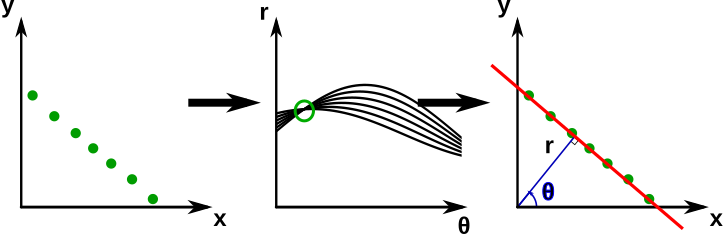
\includegraphics[width=0.45\textwidth,keepaspectratio]{HT.pdf}
        \caption[Transformation de Hough]{\label{fig::HoughTransformation}Principe de la transformation de Hough.}
      \end{figure}

      \begin{figure}[htbp]
        \centering
        \begin{subfigure}[t]{0.8\textwidth}
          \centering
          \includegraphics[width=\textwidth,keepaspectratio]{HT_real_data_track.pdf}
        \end{subfigure}\\
        \begin{subfigure}[t]{0.48\textwidth}
          \centering
          \includegraphics[width=\textwidth,keepaspectratio]{HT_real_data.pdf}
        \end{subfigure}
        \caption[Transformation de Hough dans le \TOO{}]{\label{fig::HT_real_data}Transformation de Hough appliquée dans le \TOO{}. En haut, les points reconstruits dans la vue 1 d'un événement du run 1197. En bas, l'espace de Hough associé. Les points en verts sont ceux vus par la suite comme étant sur la trace, ceux en rouge ne sont associés à aucune trace.}
      \end{figure}

      La transformation de Hough utilise l'alignement de plusieurs points pour reconstruire des traces, peu importe leur espacement. L'idée est de convertir chaque point dans un espace $x-y$ en une sinusoïdale dans un espace dit "de Hough". Les intersections de ces sinusoïdales correspondent alors à des alignements de points et donc à des traces. Il est alors possible d'identifier des traces même avec peu de coups.

      Toute droite traversant l'espace cartésien $x-y$ peut s'écrire sous une forme dite "normale", utilisant les coordonnées $r$ (distance la plus courte entre la droite et l'origine) et $\theta$ (l'angle entre la perpendiculaire à la droite passant par l'origine et l'axe des abscisses) tel que montrée sur la \autoref{fig::HoughTransformation}. L'équation d'une droite est alors
      \begin{equation}\label{eq::HT}
        r=x\cos(\theta)+y\sin(\theta)
      \end{equation}
      avec $x$ et $y$ les coordonnées des points sur la droite. La transformation de Hough consiste à prendre chaque point de l'espace initial et de tracer, dans l'espace $r-\theta$, l'équation précédente en faisant varier $\theta$ entre 0 et $\pi$. A chaque point correspond alors une sinusoïde, et comme les points sur une même droite auront les mêmes $r$ et $\theta$, les intersections de ces sinusoïdes correspondent à nos droites dans l'espace cartésien. La \autoref{fig::HT_real_data} montre ce principe avec un événement du run 1197.

      Une fois l'espace de Hough rempli, les traces sont identifiées en cherchant les maxima locaux. Une fois un maximum trouvé, une zone autour de ce dernier est ignorée afin d'éviter d'identifier plusieurs fois la même trace. Les coups correspondant à une trace lui sont alors associés en calculant leur distance à la trace à partir des $r$ et $\theta$ trouvés. Un coup est sur la trace si il est à moins de \SI{1}{\centi\meter} de cette dernière. Un ajustement linéaire est alors effectué afin de corriger les $r$ et $\theta$ pour les éventuelles imprécisions dues au binning de l'espace de Hough et l'étape d'association des coups aux traces et réitérée.

      Une fois ceci fait pour les deux vues, les traces sont appareillées en fonction des coordonnées en temps de leur premiers et derniers coups qui, pour une même trace en 3D, doit être la même dans les deux vues. Deux problèmes peuvent alors se poser avec la transformation de Hough. D'abord, si un faux coup se retrouve par hasard aligné avec une trace, il sera vu comme étant sur la trace. Et donc, la trace 2D ainsi reconstruite pourra sembler bien plus grande dans une vue que dans l'autre, empêchant l'appareillage. Ensuite, si deux traces sont présentes et que leurs droites associées se croisent, les coups proches de l'intersection seront forcément vus par la transformation de Hough comme étant sur les deux traces, même si l'une des deux se terminent avant l'intersection. Afin de remédier à cela, les premiers et derniers coups de chaque trace sont ignorés si il sont seuls ou font parti d'un amas isolé.

      Une fois les traces identifiées, la sutraction du bruit cohérent est refaite à partir des données des canaux avant soustraction du bruit, en ignorant les bins de temps le long des traces pour le calcul des moyennes. Une identification des coups est refaite et l'information $dQ/ds$ est calculée.

    \subsection{Sélection des traces et résultats}

      \begin{figure}[htbp]
        \centering
        \begin{subfigure}[t]{0.48\textwidth}
          \centering
          \includegraphics[width=\textwidth,keepaspectratio]{1197_dQds_0.pdf}
          \caption{Vue 0, run 1197, sans la seconde étape de suppression de bruit cohérent.}
        \end{subfigure}\hfill
        \begin{subfigure}[t]{0.48\textwidth}
          \centering
          \includegraphics[width=\textwidth,keepaspectratio]{1197_dQds_1.pdf}
          \caption{Vue 1,  run 1197, sans la seconde étape de suppression de bruit cohérent.}
        \end{subfigure}\\
        \begin{subfigure}[t]{0.48\textwidth}
          \centering
          \includegraphics[width=\textwidth,keepaspectratio]{1197_dQds_fromtrack_0.pdf}
          \caption{Vue 0, run 1197, avec la seconde étape de suppression de bruit cohérent.}
        \end{subfigure}\hfill
        \begin{subfigure}[t]{0.48\textwidth}
          \centering
          \includegraphics[width=\textwidth,keepaspectratio]{1197_dQds_fromtrack_1.pdf}
          \caption{Vue 1, run 1197, avec la seconde étape de suppression de bruit cohérent.}
        \end{subfigure}
        \caption[Reconstruction de la distribution de la charge déposée par unité de longueur dans le run 1197]{\label{fig::dqds_1197_Rawdatasoft}Reconstruction de la distribution de la charge déposée par unité de longueur dans le run 1197. Les deux figures du haut sont faites sans la seconde étape de bruit cohérent, une différence qui n'a aucun sens physique est observable entre les 2 vues. La figure du bas est la même distribution avec la seconde étape de suppression de bruit cohérent.}
      \end{figure}


      \begin{figure}[htbp]
        \centering
        \begin{subfigure}[t]{0.48\textwidth}
          \centering
          \includegraphics[width=\textwidth,keepaspectratio]{1199_dQds_fromtrack_0.pdf}
          \caption{Vue 0, run 1199, avec la seconde étape de suppression de bruit cohérent.}
        \end{subfigure}\hfill
        \begin{subfigure}[t]{0.48\textwidth}
          \centering
          \includegraphics[width=\textwidth,keepaspectratio]{1199_dQds_fromtrack_1.pdf}
          \caption{Vue 1, run 1199, avec la seconde étape de suppression de bruit cohérent.}
        \end{subfigure}
        \caption[Reconstruction de la distribution de la charge déposée par unité de longueur dans le run 1199]{\label{fig::dqds_1199_Rawdatasoft}Reconstruction de la distribution de la charge déposée par unité de longueur dans le run 1199 avec la seconde étape de suppression de bruit cohérent.}
      \end{figure}

      \begin{figure}[htbp]      
        \centering
        \includegraphics[width=0.6\textwidth,keepaspectratio]{dQds_fromtrack_840.pdf}
        \caption[Test de l'algorithme sur le run 840]{\label{fig::dQds_rawdatasoft_840}Reconstruction de la distribution de la charge déposée par unité de longueur dans le run 840 vue 0.}
      \end{figure}

      La transformation de Hough permet de reconstruire des traces morcelées mais droites, ce qui est nécessaire pour les runs 1197 et 1199, mais n'est pas performant du tout pour identifier une gerbe électromagnétique, hadronique ou une trace courbée. Les événements ont donc été sélectionnées à l'oeil, en regardant le résultat de la première soustraction du bruit cohérent. Afin d'éviter d'avoir à passer à travers un trop grand nombre d'événements, seuls ceux ayant passé la coupure de l'algorithme de l'équation \eqref{eq::cbr}, dont le seuil de tolérance de \numprint{0.1} a été monté à \numprint{0.3}, ont été inspectés. Les résultats en terme de distribution de $dQ/ds$ sont montrés en \autoref{fig::dqds_1197_Rawdatasoft} (deux figures du bas) pour le run 1197 et \autoref{fig::dqds_1199_Rawdatasoft} pour le run 1199. Quelques événements du run 840 ont également été analysés afin de valider l'algorithme. La \autoref{fig::dQds_rawdatasoft_840} montre les distributions de $dQ/ds$ de ces quelques événements, à comparer avec la \autoref{fig::dqds_840_842} faite à partir de la reconstruction de \gls{larsoft}. On constate que le nouvel algorithme donne une valeur de \gls{mpv} légèrement supérieure mais que les résultats sont globalement compatibles. 

\FloatBarrier

\printbibliography